
\documentclass[fleqn,addpoints]{exam}

\usepackage{graphicx}
\usepackage{booktabs}
\usepackage{float}
\usepackage{amsmath}
\usepackage{cancel}
\usepackage{polynom}
\usepackage{caption}
\usepackage{mdwlist}

\newcommand{\degree}{\ensuremath{^\circ}} 

\printanswers

\ifprintanswers 
\usepackage{2in1, lscape} 
\fi

\title{Math 115 \\ Homework 26}
\date{June 14, 2011}

\begin{document}

\maketitle

% \begin{figure}[H]
%   \centering
%   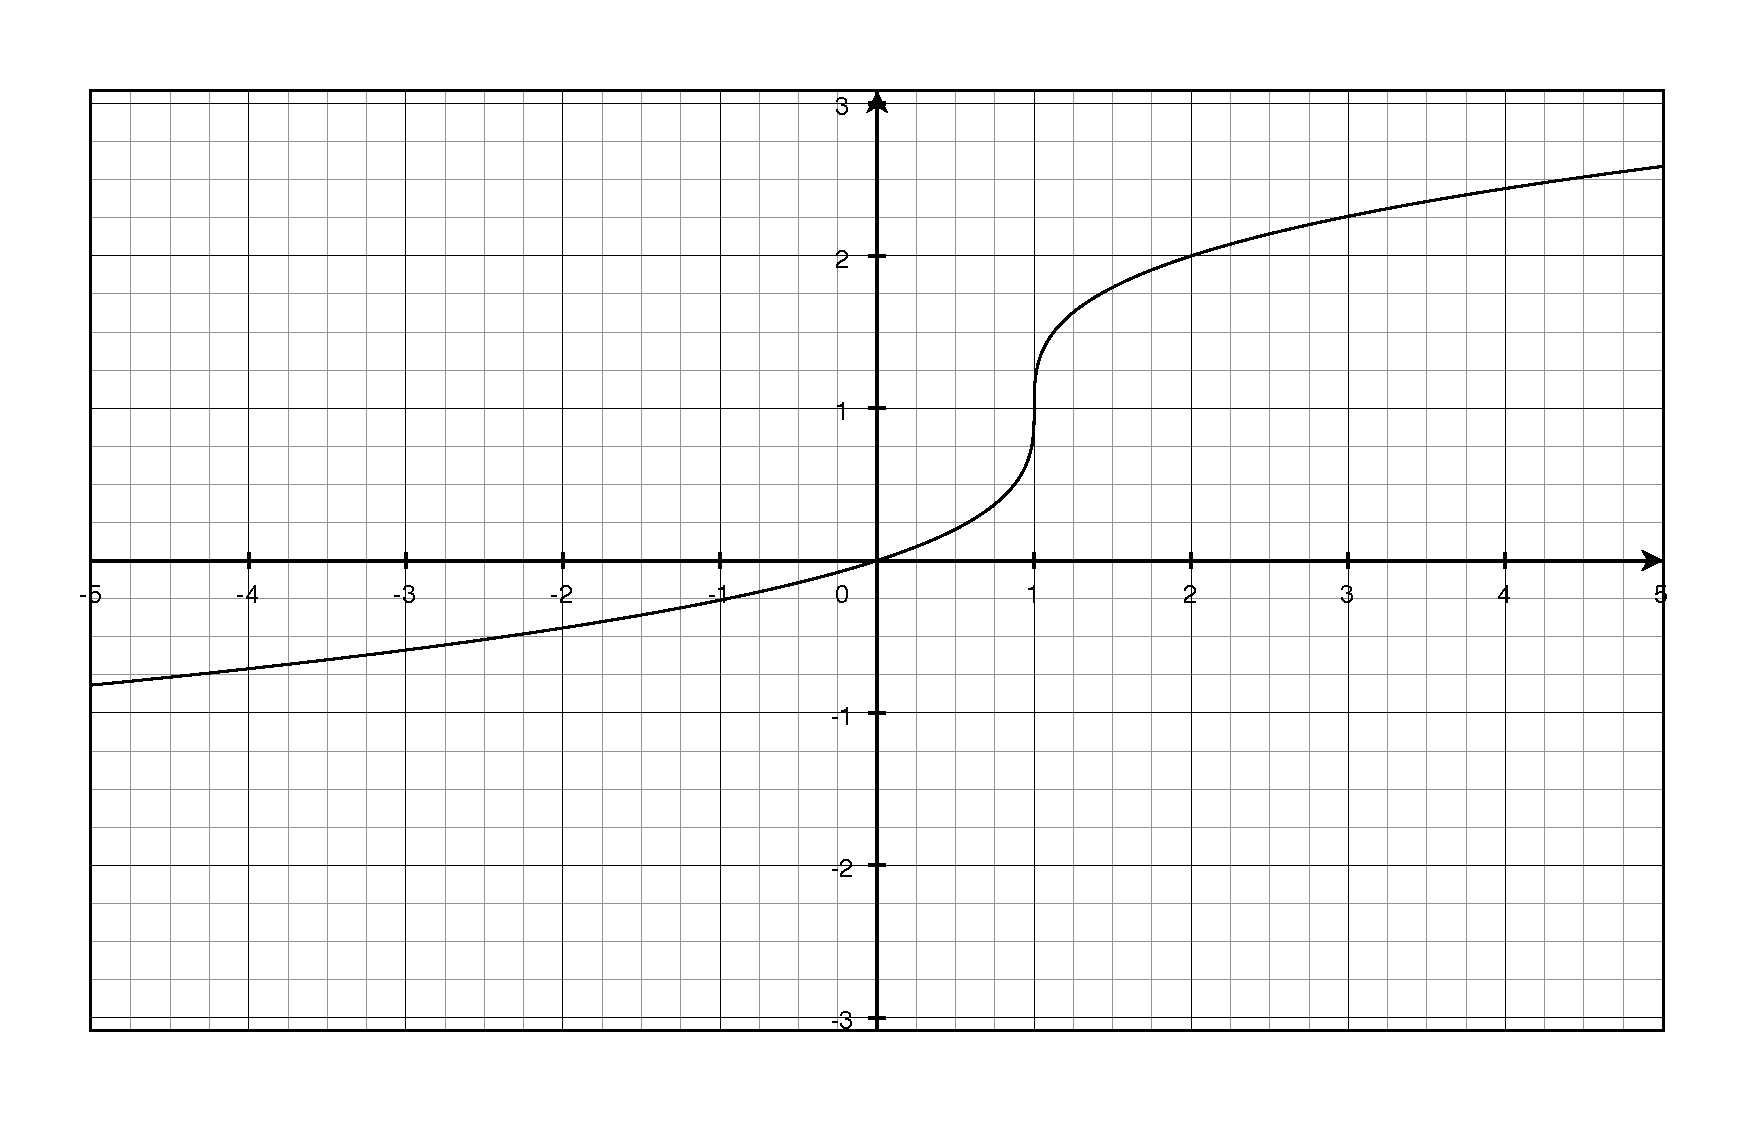
\includegraphics[scale=.3]{question7.eps}
%   \caption*{Question 7}
% \end{figure}

% \begin{tabular}{cc}
% \toprule
% period & amplitude \\
% \midrule
%   $\pi$ & $2$ \\
% \bottomrule
% \end{tabular}

\ifprintanswers
\else

\section{Administrative}

Schedule:
\begin{itemize*}
  \item June 21---Trigonometry Test
  \item June 28--July 5---Sections 10.2-10.4
  \item July---review and OU exam
\end{itemize*}

\fi

\section{Homework}
\begin{itemize*}
  \item pp. 500-502: 1-5, 17, 21-22, 27, 31-32, 37, 40, 45, 48-49
  \item pp. 507-510: 1-5, 23-24, 31, 34, 40
\end{itemize*}

\section{Extra Credit}
Page 510, question 54 and 55

\begin{description}

\item[54]
I did this one by working with both sides until they met in the middle.

The left side is:
\begin{align*}
  \frac{1}{2} bc (1 + \cos A) &=  \frac{bc}{2} \left(1 + \cfrac{b^2 + c^2 - a^2}{2 bc} \right) \\
  &= \frac{bc}{2} + \frac{b^2 + c^2 - a^2}{4} \\
  &= \frac{-a^2 + b^2 + c^2 + 2bc}{4} \\
\end{align*}

The right side is:
\begin{align*}
  \left( \frac{a+b+c}{2} \right)  \left( \frac{-a+b+c}{2} \right) &= \left( \frac{(b+c) + a}{2} \right)  \left( \frac{(b+c) - a}{2} \right) \\
  &= \frac{(b+c)^2 - a^2}{4} \\
  &= \frac{b^2 + 2bc + c^2 - a^2}{4} \\
  &= \frac{-a^2 + b^2 + c^2 + 2bc}{4} \\
\end{align*}

\item[55]
The left side is:
\begin{align*}
  \frac{1}{2} bc (1 - \cos A) &= \frac{bc}{2} \left(1 - \frac{b^2 + c^2 - a^2}{2bc} \right) \\
  &= \frac{bc}{2} - \frac{b^2 + c^2 - a^2}{4} \\
  &= \frac{a^2 - b^2 - c^2 + 2bc}{4} \\
\end{align*}

The right side is:
\begin{align*}
  \left( \frac{a-b+c}{2} \right)  \left( \frac{a+b-c}{2} \right) &= \left( \frac{a - (b-c)}{2} \right)  \left( \frac{a + (b-c)}{2} \right) \\
  &= \frac{a^2 - (b-c)^2}{4} \\
  &= \frac{a^2 - (b^2 -2bc + c^2)}{4} \\
  &= \frac{a^2 - b^2 - c^2 + 2bc}{4} \\
\end{align*}


\ifprintanswers
\section{Pages 500-502}



\item[1] 
\begin{align*}
  \frac{20}{\sin 30 \degree} &= \frac{b}{\sin 45 \degree} \\
  b &\approx 28.3 \\
  \\
  C &= 180 \degree - 30 \degree - 45 \degree = 105 \degree \\
  \\
  \frac{c}{\sin 105 \degree} &= \frac{20}{\sin 30 \degree} \\
  c &\approx 38.6 \\
\end{align*}

\item[2] 
\begin{align*}
  \frac{20}{\sin 105 \degree} &= \frac{b}{\sin 40 \degree} \\
  b &\approx 13.3 \\
  \\
  A &= 180 \degree - 105 \degree - 40 \degree = 35 \degree \\
  \\
  \frac{20}{\sin 105 \degree} &= \frac{a}{\sin 35 \degree} \\
  a &\approx 11.9 \\
\end{align*}

\item[3] 
\begin{align*}
  \frac{3.5}{\sin 25 \degree} &= \frac{b}{\sin 35 \degree} \\
  b &\approx 4.8 \\
  \\
  C &= 180 \degree - 25 \degree - 35 \degree = 120 \degree \\
  \\
  \frac{3.5}{\sin 25 \degree} &= \frac{c}{\sin 120 \degree} \\
  c &\approx 7.2 \\
\end{align*}

\item[4] 
\begin{align*}
  \frac{45}{\sin 135 \degree} &= \frac{b}{\sin 10 \degree} \\
  b &\approx 11.1 \\
  \\
  A &= 180 \degree - 135 \degree - 10 \degree = 35 \degree \\
  \\
  \frac{45}{\sin 135 \degree} &= \frac{a}{\sin 35 \degree} \\
  a &\approx 36.5 \\
\end{align*}

\item[5] 
\begin{align*}
  \frac{8}{\sin 36 \degree} &= \frac{5}{\sin B} \\
  B &\approx 21.6 \degree \\
  \\
  C &\approx 180 \degree - 36 \degree - 21.6 \degree = 122.4 \degree \\
  \\
  \frac{8}{\sin 36 \degree} &\approx \frac{c}{\sin 122.4 \degree} \\
  c &\approx 11.5 \\
\end{align*}

\item[17] 
\begin{align*}
  C &= 180 \degree - 55 \degree - 42 \degree = 83 \degree \\
  \\
  \frac{a}{\sin 55 \degree} &= \frac{0.75}{\sin 83 \degree} \\
  a &\approx 0.619 \\
  \\
  \frac{b}{\sin 42 \degree} &= \frac{0.75}{\sin 83 \degree} \\
  b &\approx 0.506 \\
\end{align*}

\item[21] 
\begin{align*}
  \frac{\sin 76 \degree}{18} &= \frac{\sin B}{20} \\
  \sin B &\approx 1.1 \\
\end{align*}

No solution.

\item[22] 
\begin{align*}
  \frac{\sin 76 \degree}{34} &= \frac{\sin B}{21} \\
  B &\approx 36.8 \degree \\
  \\ 
  C &\approx 180 \degree - 76 \degree - 36.8 \degree = 67.2 \degree \\
  \\ 
  \frac{34}{\sin 76 \degree} &\approx \frac{c}{\sin 67.2 \degree} \\
  c &\approx 32.3 \\
\end{align*}

\item[27] 
\[
  h = b \sin 36 \degree
\]

\begin{description}
\item[no solution]
$a < h$

\begin{align*}
  5 &< b \sin 36 \degree \\
  b &> 8.5 \\
\end{align*}

$b = 9$ would work.

\item[one solution]
$b < a$, so $b = 4$ would work

\item[two solutions]
$h < a < b$, so $b$ must be between 5 and 8.5.  $b = 6$ would work.

\end{description}

\item[31]
\[
  Area = \frac{1}{2} \cdot 4 \cdot 6 \cdot \sin 120 \degree = 6 \sqrt{3} \approx 10.4
\]

\item[32]
\[
  Area = \frac{1}{2} \cdot 62 \cdot 20 \cdot \sin 130 \degree \approx 474.9
\]

\item[37]
The last angle is:
\[
  180 \degree - 23 \degree - 94 \degree = 63 \degree
\]

\begin{align*}
  \frac{h}{\sin 23 \degree} &= \frac{35}{\sin 63 \degree} \\
  h &\approx 15.3 \\
\end{align*}

\item[40]
If $A$ is the angle at Canton:
\begin{align*}
  \frac{\sin A}{500} &= \frac{\sin 46 \degree}{720} \\
  A &\approx 30 \degree \\
\end{align*}

The bearing would be $90 \degree - 30 \degree = 60 \degree$ with some mysterious combination of NSEW added in to make it a bearing.

\item[45]
To find the distance to the shore we need to find one of the two distances from the boat to the lighthouse.  To do
this, we need to solve the triangle made by the two boat positions and the lighthouse.

The distance the boat travels is: $\dfrac{1}{4} \cdot 10 = 2.5$ miles.

The angles in the triangle are:
\begin{itemize}
  \item $90 \degree - 70 \degree = 20 \degree$
  \item $90 \degree + 63 \degree = 153 \degree$
  \item $180 \degree - 20 \degree - 153 \degree = 7 \degree$
\end{itemize}

Now we can find one of the other sides using the Law of Sines:
\begin{align*}
  \frac{a}{\sin 153 \degree} &= \frac{2.5}{\sin 7 \degree} \\
  a &\approx 9.3 \text{ miles}\\
\end{align*}

The distance from the shore makes a right triangle with this side as the hypotenuse, so:
\begin{align*}
  \cos 70 \degree &= \frac{d}{9.3} \\
  d &\approx 3.2 \text{ miles} \\
\end{align*}

\item[48]
true.  The longest side must always be opposite the obtuse angle.

\item[49]
false.  With two angles and a side, you can always find all the other angles and sides using the {\em Law of Sines}. 

\section{Pages 507-510}

\item[1]
\begin{align*}
  \cos A &= \frac{10^2 + 15^2 - 7^2}{2 \cdot 10 \cdot 15} \\
  A &\approx 23.1 \degree \\
  \\
  \frac{\sin B}{10} &\approx \frac{\sin 23.1 \degree}{7} \\
  B &\approx 34.0 \degree
  \\
  C &\approx 180 \degree - 23.1 \degree - 34 \degree = 122.9 \degree
\end{align*}

\item[2]
\begin{align*}
  \cos A &= \frac{3^2 + 9^2 - 8^2}{2 \cdot 3 \cdot 9} \\
  A &\approx 61.2 \degree \\
  \\
  \frac{\sin B}{3} &\approx \frac{\sin 61.2 \degree}{8} \\
  B &\approx 19.2 \degree
  \\
  C &\approx 180 \degree - 61.2 \degree - 19.2 \degree = 99.6 \degree
\end{align*}

\item[3]
\begin{align*}
  a^2 &= 15^2 + 30^2 - 2 \cdot 15 \cdot 30 \cos 30 \degree \\
  a &\approx 18.6 \\
  \\
  \frac{\sin B}{15} &\approx \frac{\sin 30 \degree}{18.6} \\
  B &\approx 23.8 \degree
  \\
  C &\approx 180 \degree - 30 \degree - 23.8 \degree = 126.2 \degree
\end{align*}

\item[4]
\begin{align*}
  c^2 &= 4.5^2 + 10^2 - 2 \cdot 4.5 \cdot 10 \cos 105 \degree \\
  c &\approx 12.0 \\
  \\
  \frac{\sin A}{10} &\approx \frac{\sin 105 \degree}{12.0} \\
  A &\approx 53.6 \degree
  \\
  B &\approx 180 \degree - 12.0 \degree - 53.8 \degree = 114.4 \degree
\end{align*}

\item[5]
\begin{align*}
  \cos A &= \frac{14^2 + 20^2 - 11^2}{2 \cdot 14 \cdot 20} \\
  A &\approx 32.0 \degree \\
  \\
  \frac{\sin B}{14} &\approx \frac{\sin 32.0 \degree}{11} \\
  B &\approx 42.4 \degree
  \\
  C &\approx 180 \degree - 32.0 \degree - 42.4 \degree = 105.6 \degree
\end{align*}

\item[23]
\begin{align*}
  s &= \frac{5 + 7 + 10}{2} = 11 \\
  area &= \sqrt{11(11-5)(11-7)(11-10)} \approx 16.2 \\
\end{align*}

\item[24]
\begin{align*}
  s &= \frac{12 + 15 + 9}{2} = 18 \\
  area &= \sqrt{18(18-12)(18-15)(18-9)} = 54 \\
\end{align*}

\item[31]
From the diagram, $B = 180 \degree - 75 \degree = 105 \degree$
\begin{align*}
  b^2 &= 220^2 + 250^2 - 2 \cdot 220 \cdot 250 \cos 105 \degree \\
  b &\approx 373 \text{ m}
\end{align*}

\item[34]
\begin{align*}
  \cos \theta &= \frac{2^2 + 3^2 - 4.5^2}{2 \cdot 2 \cdot 3} \\
  \theta &\approx 127 \degree \\
\end{align*}

\item[40]
\begin{align*}
  a^2 &= 330^2 + 420^2 - 2 \cdot 330 \cdot 420 \cos 8 \degree \\
  a &\approx 104 \text{ ft}
\end{align*}

\end{description}

\else

\vspace{3 in}

\begin{em}
% Things should be made as simple as possible, but not any simpler.
% Education is what remains after one has forgotten what one has learned in school.

I have no special talent. I am only passionately curious.

\end{em}

\vspace{.2 cm}
\hspace{1.5 cm} --Albert Einstein

\fi

\end{document}

